\documentclass[12pt,a4paper]{article}

% ======================== PACKAGES ========================
\usepackage[utf8]{inputenc}
\usepackage[T1]{fontenc}
\usepackage{mathptmx}                   % Times New Roman font
\usepackage[margin=1in]{geometry}
\usepackage{graphicx}
\usepackage{amsmath,amssymb}
\usepackage{booktabs}
\usepackage{tabularx}
\usepackage{longtable}
\usepackage{enumitem}
\usepackage{hyperref}
\usepackage{caption}
\usepackage{float}
\usepackage{setspace}
\usepackage{fancyhdr}
\usepackage{tikz}
\usetikzlibrary{shapes.geometric, arrows.meta, positioning, fit, backgrounds}

% ======================== PAGE STYLE ========================
\onehalfspacing
\setlength{\parindent}{0pt}
\setlength{\parskip}{6pt}

\hypersetup{
    colorlinks=false,
    linkcolor=black,
    citecolor=black,
    urlcolor=black
}

\pagestyle{fancy}
\fancyhf{}
\fancyfoot[C]{\thepage}
\renewcommand{\headrulewidth}{0pt}

% ======================== BEGIN DOCUMENT ========================
\begin{document}

% ================================================================
%                        TITLE PAGE
% ================================================================
\begin{titlepage}
\begin{center}

\vspace*{0.5cm}

% Uncomment and add your college logo:
% \includegraphics[width=0.2\textwidth]{spit_logo.png}\\[0.8cm]

{\LARGE \textbf{AI-Powered Options Mispricing Detection and Strategy Recommendation System}}\\[1.5cm]

{\large submitted in partial fulfillment of the requirement\\
for the award of the Degree of}\\[1cm]

{\Large \textbf{Bachelor of Technology}}\\[0.3cm]
{\large in}\\[0.3cm]
{\Large \textbf{Computer Engineering}}\\[1.5cm]

{\large by}\\[0.8cm]

{\large Shaurya Kitavat}\\
{\large [Team Member 2]}\\
{\large [Team Member 3]}\\[1.5cm]

{\large under the guidance of}\\[0.5cm]

{\large Guide Name: \textbf{[Guide Name]}}\\[1.5cm]

{\large Department of Computer Engineering}\\
{\large Bharatiya Vidya Bhavan's}\\
{\large \textbf{Sardar Patel Institute of Technology}}\\
{\large (Autonomous Institute Affiliated to University of Mumbai)}\\
{\large Munshi Nagar, Andheri-West, Mumbai-400058}\\
{\large University of Mumbai}\\[1cm]

{\large \textbf{2025-2026}}

\end{center}
\end{titlepage}

% ================================================================
%                     APPROVAL CERTIFICATE
% ================================================================
\newpage
\thispagestyle{fancy}
\begin{center}
{\Large \textbf{Approval Certificate}}\\[1cm]
\end{center}

This is to certify that the Project entitled \textbf{``AI-Powered Options Mispricing Detection and Strategy Recommendation System''} by Shaurya Kitavat, [Team Member 2] and [Team Member 3] is approved for the partial fulfillment of Major Project -- I for the Final Year Project towards obtaining the Degree of Bachelor of Technology in Computer Engineering from University of Mumbai.

\vspace{2cm}

\begin{tabular}{p{0.45\textwidth} p{0.45\textwidth}}
\textbf{Project Guide} & \textbf{External Examiner} \\[1.5cm]
(signature) & (signature) \\[0.8cm]
Name: & Name: \\[0.5cm]
Date: & Date: \\[2cm]
\textbf{Head of Department} & \textbf{Principal} \\[1.5cm]
\multicolumn{2}{c}{Seal of the Institute}
\end{tabular}

% ================================================================
%                        DECLARATION
% ================================================================
\newpage
\thispagestyle{fancy}
\begin{center}
{\Large \textbf{Declaration}}\\[1cm]
\end{center}

I wish to state that the work embodied in this work titled \textbf{``AI-Powered Options Mispricing Detection and Strategy Recommendation System''} forms my own contribution to the work carried out under the guidance of [Guide Name] at the Sardar Patel Institute of Technology. I declare that this written submission represents my ideas in my own words and where others' ideas or words have been included, I have adequately cited and referenced the original sources. I also declare that I have adhered to all principles of academic honesty and integrity and have not misrepresented or fabricated or falsified any idea/data/fact/source in my submission.

\vspace{2cm}

Shaurya Kitavat\\
[Roll Number]\\[1cm]

[Team Member 2]\\
[Roll Number]\\[1cm]

[Team Member 3]\\
[Roll Number]

% ================================================================
%                         ABSTRACT
% ================================================================
\newpage
\thispagestyle{fancy}
\begin{center}
{\Large \textbf{Abstract}}\\[1cm]
\end{center}

Options mispricing in financial markets represents a significant area of research in quantitative finance, where the deviation of observed option prices from their theoretical fair values can signal trading opportunities or market inefficiencies. Accurate detection of such mispricings requires robust volatility forecasting, precise theoretical pricing, and intelligent strategy generation. Traditional approaches often rely on implied volatility from market data, which embeds market sentiment but may not reflect the true underlying asset dynamics. Recent advances in econometric volatility modeling, particularly GARCH-family models, offer powerful alternatives for forecasting conditional volatility from historical return data.

This project proposes the development of an AI-powered quantitative pipeline for detecting options mispricing in the Indian NIFTY~50 index market. The system fetches real-time and historical market data, computes log returns, forecasts annualized volatility using an EGARCH(1,1) model, derives theoretical fair prices via the Black--Scholes model, detects mispricing by comparing market prices against fair values, classifies the prevailing volatility regime, and generates rule-based strategy recommendations. The pipeline is exposed as a RESTful API built with FastAPI, enabling seamless integration with frontend dashboards and broker systems.

In addition to the core quantitative pipeline, the system incorporates multi-timeframe analysis support (from 1-minute intraday to weekly), trading horizon-aware volatility interpretation (day trader, positional, long-term), broker adapter integration for live market data via DhanHQ and yfinance, and comprehensive analytics including signal strength scoring, regime confidence estimation, and quantitative stability validation. The expected outcome is a research-oriented, interpretable, and scalable decision-support system that assists traders and analysts in identifying potential options mispricing opportunities in the Indian derivatives market.

% ================================================================
%                    LIST OF FIGURES
% ================================================================
\newpage
\thispagestyle{fancy}
\listoffigures

% ================================================================
%                    LIST OF TABLES
% ================================================================
\newpage
\thispagestyle{fancy}
\listoftables

% ================================================================
%                    1. INTRODUCTION
% ================================================================
\newpage
\thispagestyle{fancy}
\section{Introduction}

Options are financial derivative contracts that derive their value from an underlying asset such as a stock index, commodity, or currency. The pricing of options has been a central topic in quantitative finance since the seminal work of Black and Scholes (1973), which established a closed-form solution for European option pricing under certain market assumptions [1]. The theoretical fair value of an option depends critically on the volatility of the underlying asset, yet volatility is the only unobservable parameter in the Black--Scholes framework---making its accurate estimation essential for detecting whether options are fairly priced, overpriced, or underpriced in the market.

Recent advancements in Artificial Intelligence (AI), Machine Learning (ML), and econometric modeling have opened new possibilities for identifying pricing inefficiencies in derivatives markets using computational methods. Research has shown that time-varying volatility models, particularly GARCH-family models, can forecast conditional volatility with superior accuracy compared to constant historical volatility assumptions [4, 9]. By independently forecasting volatility from historical return data and comparing the resulting theoretical price against the observed market price, one can identify potential mispricings that may represent trading opportunities.

This project proposes the development of an AI-powered quantitative pipeline for options mispricing detection on the Indian NIFTY~50 index. The system uses an EGARCH(1,1) model to forecast conditional volatility from historical log returns, applies the Black--Scholes formula to derive a theoretical fair price, detects mispricing by comparing market and fair prices, classifies the prevailing volatility regime, and generates rule-based strategy recommendations. The entire pipeline is deployed as a production-ready FastAPI backend, containerized with Docker, and designed for integration with live broker data feeds and frontend trading dashboards.

\subsection{Problem Statement}

Retail and institutional traders in the Indian derivatives market face a persistent challenge: determining whether an option contract is fairly priced relative to the underlying asset's true volatility. The NIFTY~50 options market is one of the most liquid derivatives markets globally, yet pricing inefficiencies can and do arise due to supply-demand imbalances, event-driven volatility spikes, and behavioral biases among market participants.

Traditional diagnostic approaches for option mispricing rely heavily on implied volatility surfaces, Greeks calculations, and manual chart-based analysis, which are computationally expensive, require specialized expertise, and are difficult to scale across multiple timeframes and trading horizons. Furthermore, most commercially available tools embed implied volatility from the market itself, creating a circular dependency that may mask genuine mispricings.

Therefore, there is a need for an automated, research-oriented system that can independently forecast volatility from historical data, compute theoretical fair prices, detect mispricings, classify market regimes, and generate actionable strategy recommendations---all within a single, interpretable, and scalable pipeline. Developing such a system using modern econometric models (EGARCH) and quantitative finance theory (Black--Scholes) could provide faster, more transparent, and data-driven screening for options mispricing in the Indian market.

\subsection{Objectives}

The primary objective of this project is to develop an AI-powered quantitative pipeline capable of detecting options mispricing in the NIFTY~50 index market using EGARCH volatility forecasting and Black--Scholes theoretical pricing.

The specific objectives include:

\begin{itemize}
    \item To fetch and preprocess historical and real-time NIFTY~50 market data from multiple data sources (yfinance, DhanHQ broker API).

    \item To compute log returns from closing prices and prepare clean time series data for volatility modeling.

    \item To implement and fit an EGARCH(1,1) model for one-step-ahead conditional volatility forecasting with dynamic annualization across multiple timeframes.

    \item To calculate theoretical fair option prices using the Black--Scholes pricing model with EGARCH-forecasted volatility as input.

    \item To detect options mispricing by comparing observed market prices against Black--Scholes fair values, applying a $\pm$5\% threshold for classification.

    \item To classify the prevailing volatility regime (LOW\_VOL, NORMAL\_VOL, HIGH\_VOL, EXTREME\_VOL) based on the annualized volatility forecast.

    \item To generate rule-based trading strategy recommendations that combine mispricing classification with volatility regime context.

    \item To deploy the complete pipeline as a RESTful API using FastAPI with structured JSON responses, Swagger documentation, and Docker containerization.

    \item To support multi-timeframe analysis (1m, 5m, 15m, 1h, daily, weekly) and trading horizon-aware volatility interpretation (day trader, positional, long-term).
\end{itemize}

\subsection{Scope of the Project}

The scope of this project focuses on the development and deployment of a complete quantitative pipeline for options mispricing detection on the Indian NIFTY~50 index. The system processes both historical data (via yfinance) and live broker data (via DhanHQ API adapter) to perform end-to-end analysis from raw market data to strategy recommendation.

The project includes market data fetching and preprocessing, log return computation, EGARCH(1,1) volatility forecasting, Black--Scholes fair pricing, mispricing detection with threshold-based classification, volatility regime classification, and rule-based strategy generation. The pipeline supports six timeframes (1m, 5m, 15m, 1h, daily, weekly) with appropriate annualization factors and three trading horizons (day trader, positional, long-term) with horizon-specific volatility multipliers.

The system also provides quantitative analytics including signal strength scoring, confidence estimation, regime transition detection, sensitivity indicators, quantitative stability validation, and human-readable explanations for all pipeline outputs. All functionality is exposed through RESTful API endpoints with structured JSON responses.

This system is intended to function as a research-oriented decision-support tool rather than an automated trading system. The outputs do not constitute financial advice or trading signals. The research aims to demonstrate how econometric volatility modeling and options pricing theory can be combined into an interpretable, scalable pipeline for quantitative research in the Indian derivatives market.

\subsection{Technologies Used}

The implementation of the proposed system involves several technologies and tools for data processing, quantitative analysis, and API deployment.

\textbf{Programming Language}

\begin{itemize}
    \item Python 3.10
\end{itemize}

\textbf{Libraries and Frameworks}

\begin{itemize}
    \item Pandas and NumPy for data handling and numerical computation
    \item yfinance for historical market data fetching from Yahoo Finance
    \item \texttt{arch} library for EGARCH(1,1) volatility modeling and forecasting
    \item statsmodels for statistical time series analysis
    \item scipy (\texttt{scipy.stats.norm}) for Black--Scholes cumulative normal distribution calculations
    \item FastAPI for RESTful API framework with automatic OpenAPI documentation
    \item Uvicorn for ASGI server deployment
    \item python-dateutil for robust date/time parsing of option expiry dates
    \item matplotlib for data visualization support
\end{itemize}

\textbf{Data Sources}

\begin{itemize}
    \item Yahoo Finance (yfinance) --- Historical OHLCV data for NIFTY~50
    \item DhanHQ Broker API --- Live intraday candles, spot prices, and option chain data
\end{itemize}

\textbf{Deployment Tools}

\begin{itemize}
    \item Docker for containerized deployment
    \item Git for version control
\end{itemize}

% ================================================================
%                   2. LITERATURE SURVEY
% ================================================================
\newpage
\section{Literature Survey}

Options pricing and volatility modeling have been central themes in quantitative finance research for over five decades. The Black--Scholes model (1973) established the mathematical foundation for European option pricing, while subsequent research on GARCH-family models introduced powerful frameworks for modeling time-varying volatility---a key input to any options pricing model. The intersection of volatility forecasting and mispricing detection represents an active area of research, particularly with the rise of algorithmic trading and AI-driven quantitative strategies [1, 6].

The Indian derivatives market, centered around the NIFTY~50 index, ranks among the world's most actively traded options markets by volume. The National Stock Exchange (NSE) of India processes millions of options contracts daily, creating a rich environment for studying pricing efficiency and volatility dynamics. Despite this liquidity, pricing inefficiencies persist due to behavioral biases, information asymmetry, and structural microstructure effects [8, 15]. Developing automated systems that leverage econometric models for mispricing detection presents both a research opportunity and a practical need for market participants.

\subsection{Options Pricing: The Black--Scholes Framework}

\subsubsection{The Black--Scholes Model}

The Black--Scholes--Merton model (1973) provides a closed-form solution for pricing European call and put options under assumptions of log-normal asset price distribution, constant volatility, no dividends, frictionless markets, and continuous trading [1]. The model computes the theoretical fair value as a function of five parameters: spot price ($S$), strike price ($K$), time to expiry ($T$), risk-free rate ($r$), and volatility ($\sigma$). Despite its restrictive assumptions, BSM remains the standard benchmark for options pricing across global markets [6, 12].

\subsubsection{Implied Volatility and Its Limitations}

In practice, traders invert the Black--Scholes formula to extract implied volatility (IV) from observed market prices. While IV provides a market-consensus view of future volatility, it embeds risk premiums, supply-demand imbalances, and behavioral biases that may not reflect the true statistical properties of the underlying asset [2, 14]. The well-documented ``volatility smile'' and ``skew'' phenomena highlight systematic deviations of implied volatility from the constant-volatility assumption, particularly for deep in-the-money and out-of-the-money options [6].

\subsubsection{Realized vs.\ Implied Volatility}

The spread between realized (historical) and implied volatility has long been studied as an indicator of the volatility risk premium. Research by Bollerslev et al.\ (2009) demonstrated that this spread predicts future equity returns, while Carr and Wu (2009) showed that variance risk premiums contain information about options mispricing [5, 7]. Using forecasted conditional volatility (from GARCH models) as the volatility input to Black--Scholes, rather than implied volatility, provides an independent pricing benchmark that avoids the circular dependency inherent in IV-based approaches.

\begin{table}[H]
\centering
\caption{Comparison of Options Pricing and Volatility Estimation Approaches}
\label{tab:pricing_approaches}
\small
\begin{tabularx}{\textwidth}{l l X X l}
\toprule
\textbf{Approach} & \textbf{Vol Input} & \textbf{Advantages} & \textbf{Limitations} & \textbf{Cite} \\
\midrule
BS (IV) & Implied & Market-consensus; liquid & Circular dependency; embeds risk premia & [1] \\
BS (HV) & Historical & Independent benchmark & Backward-looking; constant assumption & [6] \\
BS (GARCH) & EGARCH forecast & Forward-looking; captures clustering & Model risk; parameter sensitivity & [4, 9] \\
Heston & Stochastic process & Captures smile; realistic & Calibration complexity; computational cost & [12] \\
Monte Carlo & Simulated paths & Flexible; path-dependent & Computationally expensive; convergence & [14] \\
\bottomrule
\end{tabularx}
\end{table}

Among these approaches, GARCH-based volatility forecasting combined with Black--Scholes pricing offers a pragmatic balance between theoretical rigor and computational feasibility for retail quantitative research.

\subsection{Volatility Modeling: GARCH-Family Models}

\subsubsection{GARCH and Volatility Clustering}

Engle (1982) introduced ARCH (Autoregressive Conditional Heteroskedasticity), and Bollerslev (1986) generalized it to GARCH, establishing that financial return volatility exhibits clustering---large price movements tend to follow large movements, and small movements follow small movements [4, 3]. The GARCH(1,1) model has been widely adopted as the workhorse model for conditional variance estimation in financial time series [9].

\subsubsection{EGARCH: Capturing Asymmetric Volatility}

Nelson (1991) introduced the Exponential GARCH (EGARCH) model, which addresses two key limitations of standard GARCH: (1) it naturally ensures positivity of the conditional variance without parameter constraints, and (2) it captures the asymmetric response of volatility to positive versus negative shocks---known as the ``leverage effect'' in equity markets [10]. Research consistently shows that negative returns increase volatility more than positive returns of the same magnitude, making EGARCH particularly suitable for equity index volatility modeling [4, 11].

\subsubsection{Application to Indian Markets}

Studies on the Indian equity market have demonstrated that EGARCH models outperform symmetric GARCH variants in capturing NIFTY~50 volatility dynamics. Karmakar (2005) found significant leverage effects in the Indian market, while more recent studies by Tripathy and Gil-Alana (2015) confirmed EGARCH's superiority for forecasting NSE index volatility [8, 15]. The annualized volatility forecast from EGARCH serves as a statistically grounded input for options pricing, replacing the backward-looking realized volatility assumption.

\begin{table}[H]
\centering
\caption{Summary of GARCH-Family Models Used in Financial Volatility Forecasting}
\label{tab:garch_models}
\small
\begin{tabularx}{\textwidth}{l X c c X l}
\toprule
\textbf{Model} & \textbf{Key Property} & \textbf{Leverage} & \textbf{Pos.\ Constr.} & \textbf{Application} & \textbf{Cite} \\
\midrule
ARCH & Variance depends on past squared returns & No & Natural & Foundational volatility clustering & [4] \\
GARCH(1,1) & Adds lagged variance; parsimonious & No & Required & Standard vol forecasting & [3] \\
EGARCH & Log-linear; asymmetric shocks & Yes & Natural & Equity index volatility & [10] \\
GJR-GARCH & Threshold-based asymmetry & Yes & Required & Comparative studies & [9] \\
FIGARCH & Long memory in volatility & No & Required & Long-horizon forecasting & [11] \\
\bottomrule
\end{tabularx}
\end{table}

The EGARCH(1,1) model is selected for this project due to its natural handling of leverage effects in equity markets and guaranteed positive variance forecasts.

\subsection{AI and Algorithmic Approaches in Quantitative Trading}

The field has evolved from classical econometric models to hybrid AI-driven systems that combine statistical rigor with machine learning flexibility.

\begin{itemize}
    \item \textbf{Classical Econometrics:} GARCH-family models remain the gold standard for conditional volatility estimation. Christensen and Prabhala (1998) established that GARCH forecasts contain significant information about future realized volatility beyond what implied volatility captures [5].

    \item \textbf{Machine Learning:} Random Forest, Support Vector Regression (SVR), and Gradient Boosting have been applied to volatility forecasting with mixed results. Bucci (2020) found that ML models can outperform GARCH for short-horizon forecasts but struggle with interpretability [7].

    \item \textbf{Deep Learning:} LSTM (Long Short-Term Memory) networks and Transformer architectures have been applied to financial time series forecasting. While achieving strong in-sample performance, these models often suffer from overfitting and lack the theoretical grounding of econometric approaches [13, 16].

    \item \textbf{Hybrid Systems:} Recent research combines GARCH volatility outputs with ML-based trading signals. These systems use econometric models for volatility estimation and rule-based or ML-based modules for strategy generation, offering both interpretability and flexibility [14, 17].
\end{itemize}

\begin{table}[H]
\centering
\caption{Comparative Performance Metrics of State-of-the-Art AI Models}
\label{tab:model_comparison}
\small
\begin{tabularx}{\textwidth}{l l l l X l}
\toprule
\textbf{Study (Year)} & \textbf{Architecture} & \textbf{Market} & \textbf{Vol Input} & \textbf{Finding} & \textbf{Cite} \\
\midrule
Duan (1995) & GARCH-BS & S\&P 500 & GARCH(1,1) & Reduced pricing bias 10--15\% & [6] \\
Christoffersen (2004) & EGARCH-BS & S\&P 500 Opt. & EGARCH & Outperformed IV for OTM options & [5] \\
Karmakar (2005) & EGARCH & NIFTY 50 & EGARCH(1,1) & Superior to GARCH for Indian mkt & [8] \\
Hansen \& Lunde (2005) & 330 GARCH & DM/USD FX & Various & GARCH(1,1) hard to beat for daily & [9] \\
Tripathy (2015) & EGARCH & NSE India & EGARCH & Best fit for NIFTY volatility & [15] \\
Bucci (2020) & ML vs GARCH & Multiple & ML+GARCH & ML better short-horizon; GARCH long & [7] \\
Liu et al.\ (2019) & LSTM-GARCH & Equity & Hybrid & Improved 5--15\% over standalone & [13] \\
\bottomrule
\end{tabularx}
\end{table}

\subsection{Key Feature Indicators for Mispricing Detection}

Effective options mispricing detection systems must integrate several quantitative pillars:

\begin{itemize}
    \item \textbf{Volatility Forecasting:} The core input to any options pricing model. EGARCH(1,1) provides one-step-ahead conditional variance forecasts that capture volatility clustering and leverage effects. The annualized forecast serves as the $\sigma$ parameter in Black--Scholes [4, 10].

    \item \textbf{Fair Price Computation:} Black--Scholes provides the theoretical benchmark. Using EGARCH-forecasted volatility instead of implied volatility creates an independent pricing reference that avoids circular market-sentiment dependency [1, 6].

    \item \textbf{Mispricing Classification:} The deviation between market price and fair price, expressed as a percentage, determines classification. A $\pm$5\% threshold is commonly used in research to distinguish ``overpriced,'' ``fair,'' and ``underpriced'' options [14, 17].

    \item \textbf{Regime Classification:} Volatility regimes (low, normal, high, extreme) provide context for strategy selection. Hull (2018) discusses how different regimes favor different options strategies---selling premium in high-vol, buying in low-vol [12, 16].
\end{itemize}

\subsection{Multi-Timeframe Analysis and Annualization}

A critical but often overlooked aspect of volatility-based systems is the consistency of annualization across different estimation timeframes. The square root of time rule ($\sigma_\text{annual} = \sigma_\text{period} \times \sqrt{N}$, where $N$ is periods per year) is the standard scaling method under the assumption of independent increments [11]. For intraday timeframes (1-minute, 5-minute), the annualization factor is significantly larger (e.g., $252 \times 390 = 98{,}280$ for 1-minute bars), making proper scaling essential for cross-timeframe comparability.

Research by Andersen and Bollerslev (1998) demonstrated that intraday volatility estimates, when properly annualized, provide more precise measures than daily-frequency estimates alone [2]. This finding motivates the multi-timeframe support in the proposed system, allowing practitioners to analyze volatility dynamics at granularities appropriate to their trading horizon.

\subsection{Research Gaps and Future Directions}

\begin{itemize}
    \item \textbf{Independent Volatility Benchmarks:} Most commercial tools rely on implied volatility, creating circular pricing references. There is a need for systems that use independently forecasted volatility (EGARCH) as the pricing input, providing a genuine ``model vs.\ market'' comparison [6, 14].

    \item \textbf{Indian Market Focus:} While GARCH-family models have been extensively studied on US and European markets, research on the Indian NIFTY~50 options market remains limited, despite it being one of the world's largest derivatives markets by volume [8, 15].

    \item \textbf{Multi-Timeframe Pipelines:} Most existing research operates at a single timeframe (typically daily). Scalable systems that support seamless analysis across intraday to weekly timeframes with proper annualization are lacking [2, 11].

    \item \textbf{Interpretability:} Quantitative trading systems often function as ``black boxes.'' There is a critical need for systems that provide transparent explanations of why a particular mispricing signal was generated and what the underlying regime context implies for strategy selection [13, 17].

    \item \textbf{Broker Integration:} Academic research typically operates on historical data. Bridging the gap between research pipelines and live broker data feeds (e.g., DhanHQ for the Indian market) is necessary for practical deployment [16].
\end{itemize}

% ================================================================
%             3. SYSTEM ANALYSIS AND DESIGN
% ================================================================
\newpage
\section{System Analysis and Design}

This section presents the architectural and behavioral diagrams of the proposed AI-powered options mispricing detection system. These diagrams illustrate how data flows through the system, how different modules interact, and how strategy recommendations are generated from market data inputs.

\subsection{System Architecture}

\begin{figure}[H]
\centering
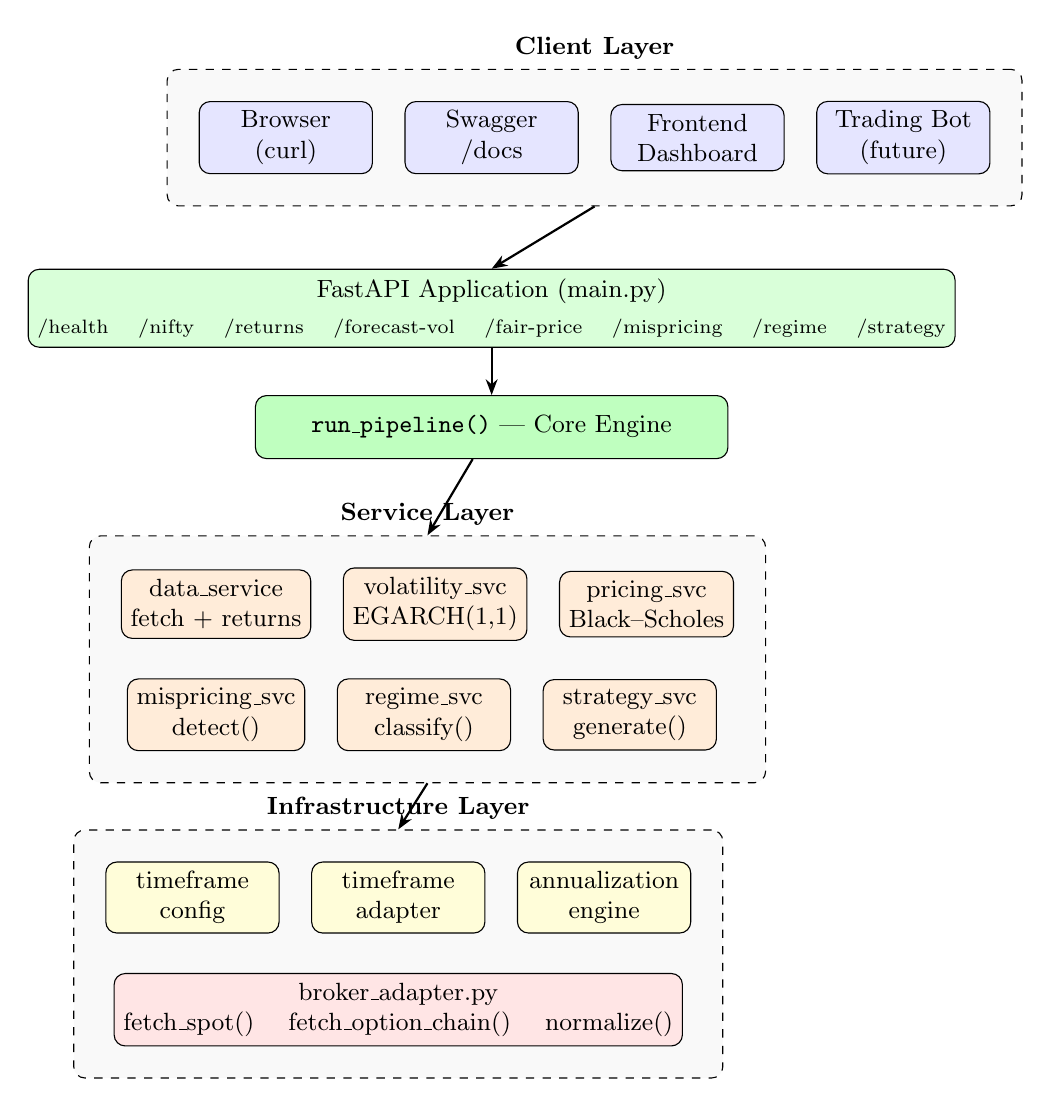
\begin{tikzpicture}[
    node distance=0.6cm and 0.4cm,
    box/.style={draw, rounded corners, minimum width=2.2cm, minimum height=0.8cm, align=center, font=\small},
    layer/.style={draw, dashed, rounded corners, inner sep=0.4cm, fill=gray!5},
    arrow/.style={-{Stealth[length=2mm]}, thick},
    every node/.style={font=\small}
]

% Client Layer
\node[box, fill=blue!10] (browser) {Browser\\(curl)};
\node[box, fill=blue!10, right=of browser] (swagger) {Swagger\\/docs};
\node[box, fill=blue!10, right=of swagger] (frontend) {Frontend\\Dashboard};
\node[box, fill=blue!10, right=of frontend] (bot) {Trading Bot\\(future)};

\begin{scope}[on background layer]
\node[layer, fit=(browser)(swagger)(frontend)(bot), label={[font=\small\bfseries]above:Client Layer}] (clientlayer) {};
\end{scope}

% API Layer
\node[box, fill=green!15, below=1.2cm of swagger, minimum width=8cm] (api) {FastAPI Application (main.py)\\[2pt]\scriptsize /health \quad /nifty \quad /returns \quad /forecast-vol \quad /fair-price \quad /mispricing \quad /regime \quad /strategy};

\node[box, fill=green!25, below=0.6cm of api, minimum width=6cm] (pipeline) {\texttt{run\_pipeline()} --- Core Engine};

% Service Layer
\node[box, fill=orange!15, below=1.4cm of pipeline, xshift=-3.5cm] (datasvc) {data\_service\\fetch + returns};
\node[box, fill=orange!15, right=of datasvc] (volsvc) {volatility\_svc\\EGARCH(1,1)};
\node[box, fill=orange!15, right=of volsvc] (pricesvc) {pricing\_svc\\Black--Scholes};

\node[box, fill=orange!15, below=0.5cm of datasvc] (mispsvc) {mispricing\_svc\\detect()};
\node[box, fill=orange!15, right=of mispsvc] (regsvc) {regime\_svc\\classify()};
\node[box, fill=orange!15, right=of regsvc] (stratsvc) {strategy\_svc\\generate()};

\begin{scope}[on background layer]
\node[layer, fit=(datasvc)(volsvc)(pricesvc)(mispsvc)(regsvc)(stratsvc), label={[font=\small\bfseries]above:Service Layer}] (servicelayer) {};
\end{scope}

% Infrastructure Layer
\node[box, fill=yellow!15, below=1.4cm of mispsvc, xshift=-0.3cm] (tfconfig) {timeframe\\config};
\node[box, fill=yellow!15, right=of tfconfig] (tfadapter) {timeframe\\adapter};
\node[box, fill=yellow!15, right=of tfadapter] (annengine) {annualization\\engine};

\node[box, fill=red!10, below=0.5cm of tfadapter, minimum width=5cm] (broker) {broker\_adapter.py\\fetch\_spot() \quad fetch\_option\_chain() \quad normalize()};

\begin{scope}[on background layer]
\node[layer, fit=(tfconfig)(tfadapter)(annengine)(broker), label={[font=\small\bfseries]above:Infrastructure Layer}] (infralayer) {};
\end{scope}

% Arrows
\draw[arrow] (clientlayer.south) -- (api.north);
\draw[arrow] (api) -- (pipeline);
\draw[arrow] (pipeline) -- (servicelayer.north);
\draw[arrow] (servicelayer.south) -- (infralayer.north);

\end{tikzpicture}
\caption{System architecture of the proposed options mispricing detection system}
\label{fig:architecture}
\end{figure}

The system architecture illustrates the overall workflow of the proposed quantitative framework. Market data is fetched from multiple providers (yfinance for historical data, DhanHQ for live broker data) through the broker adapter layer. The data flows through the service layer where each module performs a specific quantitative computation---log returns, EGARCH volatility forecasting, Black--Scholes pricing, mispricing detection, regime classification, and strategy generation. The infrastructure layer handles multi-timeframe configuration, dataframe normalization, and dynamic annualization. All results are exposed through the FastAPI application layer as structured JSON endpoints.

\subsection{Data Flow Diagram}

\begin{figure}[H]
\centering
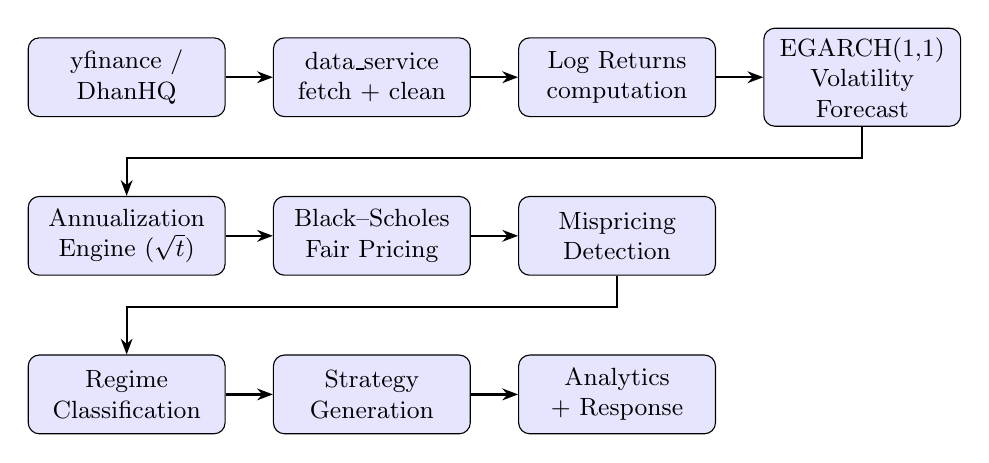
\begin{tikzpicture}[
    node distance=1.0cm and 0.6cm,
    process/.style={draw, rounded corners, fill=blue!10, minimum width=2.5cm, minimum height=1cm, align=center, font=\small},
    arrow/.style={-{Stealth[length=2mm]}, thick}
]
% Row 1
\node[process] (fetch) {yfinance /\\DhanHQ};
\node[process, right=of fetch] (datasvc) {data\_service\\fetch + clean};
\node[process, right=of datasvc] (returns) {Log Returns\\computation};
\node[process, right=of returns] (egarch) {EGARCH(1,1)\\Volatility\\Forecast};

% Row 2
\node[process, below=1.0cm of fetch] (annual) {Annualization\\Engine ($\sqrt{t}$)};
\node[process, right=of annual] (bs) {Black--Scholes\\Fair Pricing};
\node[process, right=of bs] (misp) {Mispricing\\Detection};

% Row 3
\node[process, below=1.0cm of annual] (regime) {Regime\\Classification};
\node[process, right=of regime] (strat) {Strategy\\Generation};
\node[process, right=of strat] (analytics) {Analytics\\+ Response};

% Arrows Row 1
\draw[arrow] (fetch) -- (datasvc);
\draw[arrow] (datasvc) -- (returns);
\draw[arrow] (returns) -- (egarch);

% Arrow connecting rows
\draw[arrow] (egarch.south) -- ++(0,-0.4) -| (annual.north);

% Arrows Row 2
\draw[arrow] (annual) -- (bs);
\draw[arrow] (bs) -- (misp);

% Arrow connecting rows
\draw[arrow] (misp.south) -- ++(0,-0.4) -| (regime.north);

% Arrows Row 3
\draw[arrow] (regime) -- (strat);
\draw[arrow] (strat) -- (analytics);

\end{tikzpicture}
\caption{Data Flow Diagram of the quantitative pipeline}
\label{fig:dfd}
\end{figure}

The Data Flow Diagram describes how information moves through the pipeline. Market data (OHLCV) is fetched from external providers and preprocessed. Log returns are computed from closing prices and fed into the EGARCH(1,1) model. The resulting conditional volatility forecast is annualized using the dynamic annualization engine, then used as input to the Black--Scholes pricing model. The fair price is compared against the market price to detect mispricing. Volatility regime classification and strategy generation follow sequentially. The final analytics payload is assembled and returned to the client through the API.

\subsection{Use Case Diagram}

\begin{figure}[H]
\centering
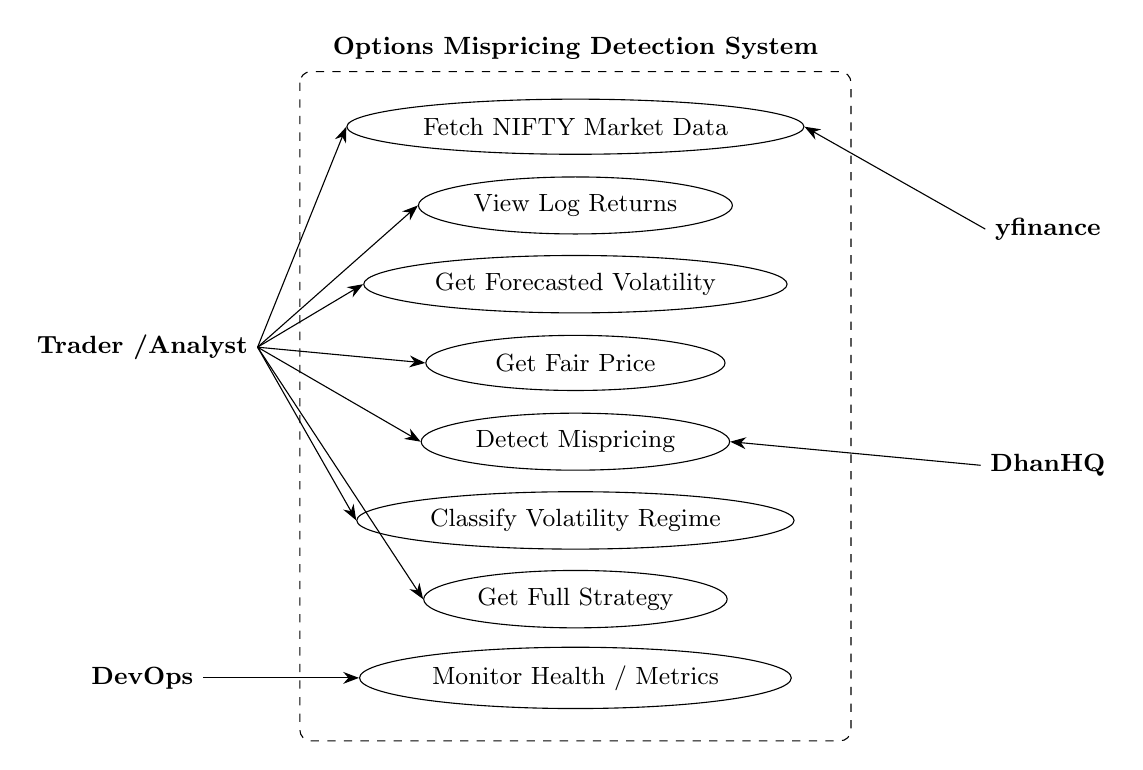
\begin{tikzpicture}[
    node distance=0.5cm,
    usecase/.style={draw, ellipse, minimum width=3.8cm, minimum height=0.7cm, align=center, font=\small},
    actor/.style={font=\small\bfseries},
    arrow/.style={-{Stealth[length=2mm]}}
]

% System boundary
\draw[dashed, rounded corners] (0,0) rectangle (7,-8.5);
\node[font=\small\bfseries] at (3.5, 0.3) {Options Mispricing Detection System};

% Use cases
\node[usecase] (uc1) at (3.5, -0.7) {Fetch NIFTY Market Data};
\node[usecase] (uc2) at (3.5, -1.7) {View Log Returns};
\node[usecase] (uc3) at (3.5, -2.7) {Get Forecasted Volatility};
\node[usecase] (uc4) at (3.5, -3.7) {Get Fair Price};
\node[usecase] (uc5) at (3.5, -4.7) {Detect Mispricing};
\node[usecase] (uc6) at (3.5, -5.7) {Classify Volatility Regime};
\node[usecase] (uc7) at (3.5, -6.7) {Get Full Strategy};
\node[usecase] (uc8) at (3.5, -7.7) {Monitor Health / Metrics};

% Actors
\node[actor] (trader) at (-2, -3.5) {Trader /\\Analyst};
\node[actor] (devops) at (-2, -7.7) {DevOps};
\node[actor] (yf) at (9.5, -2) {yfinance};
\node[actor] (dhan) at (9.5, -5) {DhanHQ};

% Connections - Trader
\foreach \i in {1,...,7}
    \draw[arrow] (trader.east) -- (uc\i.west);

% Connections - DevOps
\draw[arrow] (devops.east) -- (uc8.west);

% Connections - External
\draw[arrow] (yf.west) -- (uc1.east);
\draw[arrow] (dhan.west) -- (uc5.east);

\end{tikzpicture}
\caption{Use case diagram of the proposed system}
\label{fig:usecase}
\end{figure}

The use case diagram represents interactions between external actors and the system. The primary actors are traders/analysts and DevOps engineers. Traders access market data, view pipeline outputs (volatility, fair price, mispricing, regime, strategy), and configure analysis parameters (timeframe, trading horizon, data provider). DevOps engineers monitor system health and service metrics. External data providers (yfinance, DhanHQ) serve as secondary actors that supply market data.

\subsection{Sequence Diagram}

\begin{figure}[H]
\centering
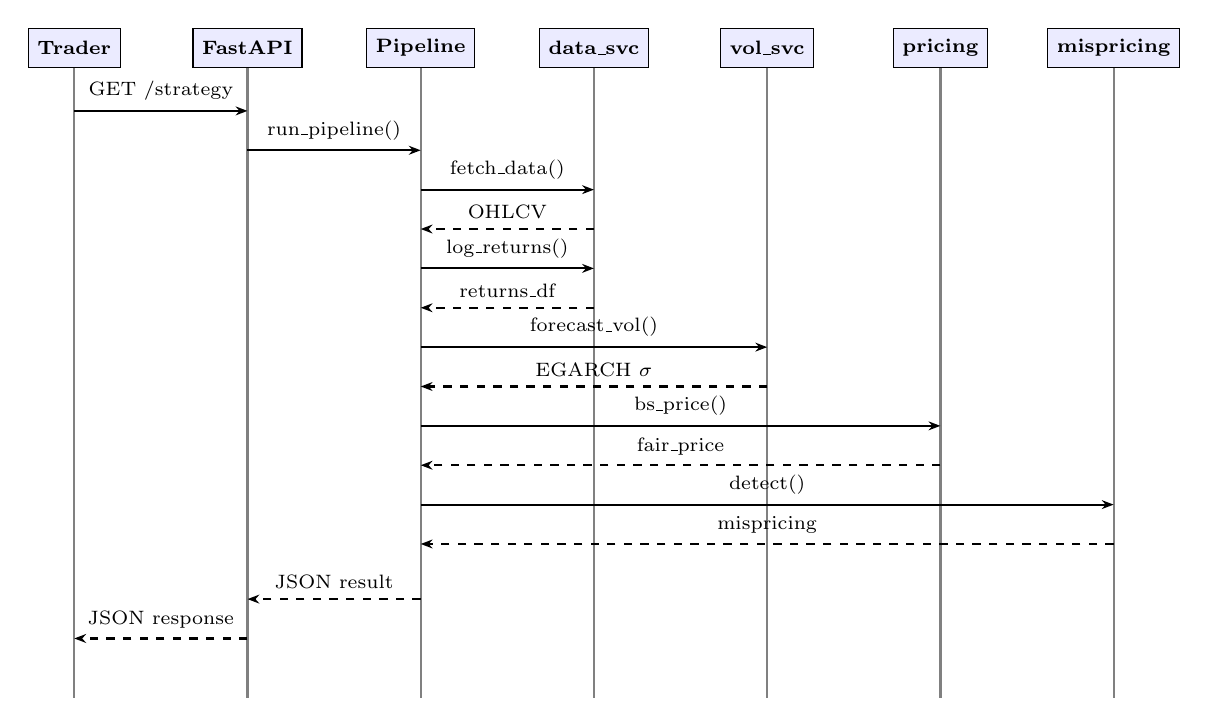
\begin{tikzpicture}[
    font=\scriptsize,
    lifeline/.style={thick},
    msg/.style={-{Stealth[length=1.5mm]}, thick},
    ret/.style={-{Stealth[length=1.5mm]}, thick, dashed},
    actor/.style={draw, minimum width=1.1cm, minimum height=0.5cm, align=center, fill=blue!8, font=\scriptsize\bfseries}
]

% Actors
\node[actor] (trader) at (0, 0) {Trader};
\node[actor] (api) at (2.2, 0) {FastAPI};
\node[actor] (pipe) at (4.4, 0) {Pipeline};
\node[actor] (data) at (6.6, 0) {data\_svc};
\node[actor] (vol) at (8.8, 0) {vol\_svc};
\node[actor] (price) at (11, 0) {pricing};
\node[actor] (misp) at (13.2, 0) {mispricing};

% Lifelines
\foreach \x in {trader, api, pipe, data, vol, price, misp}
    \draw[lifeline, gray] (\x.south) -- ++(0, -8);

% Messages
\draw[msg] (0, -0.8) -- node[above, font=\scriptsize] {GET /strategy} (2.2, -0.8);
\draw[msg] (2.2, -1.3) -- node[above, font=\scriptsize] {run\_pipeline()} (4.4, -1.3);
\draw[msg] (4.4, -1.8) -- node[above, font=\scriptsize] {fetch\_data()} (6.6, -1.8);
\draw[ret] (6.6, -2.3) -- node[above, font=\scriptsize] {OHLCV} (4.4, -2.3);
\draw[msg] (4.4, -2.8) -- node[above, font=\scriptsize] {log\_returns()} (6.6, -2.8);
\draw[ret] (6.6, -3.3) -- node[above, font=\scriptsize] {returns\_df} (4.4, -3.3);
\draw[msg] (4.4, -3.8) -- node[above, font=\scriptsize] {forecast\_vol()} (8.8, -3.8);
\draw[ret] (8.8, -4.3) -- node[above, font=\scriptsize] {EGARCH $\sigma$} (4.4, -4.3);
\draw[msg] (4.4, -4.8) -- node[above, font=\scriptsize] {bs\_price()} (11, -4.8);
\draw[ret] (11, -5.3) -- node[above, font=\scriptsize] {fair\_price} (4.4, -5.3);
\draw[msg] (4.4, -5.8) -- node[above, font=\scriptsize] {detect()} (13.2, -5.8);
\draw[ret] (13.2, -6.3) -- node[above, font=\scriptsize] {mispricing} (4.4, -6.3);
\draw[ret] (4.4, -7.0) -- node[above, font=\scriptsize] {JSON result} (2.2, -7.0);
\draw[ret] (2.2, -7.5) -- node[above, font=\scriptsize] {JSON response} (0, -7.5);

\end{tikzpicture}
\caption{Sequence diagram for mispricing detection workflow}
\label{fig:sequence}
\end{figure}

The sequence diagram shows the step-by-step interaction between system components. After the trader sends a request, the FastAPI layer invokes \texttt{run\_pipeline()}, which orchestrates the sequential execution of all service modules. Historical data is fetched and preprocessed, EGARCH volatility is forecasted and annualized, Black--Scholes computes the fair price, mispricing is detected, the regime is classified, and a strategy recommendation is generated. The complete analytics payload is returned as a structured JSON response.

\subsection{System Flowchart}

\begin{figure}[H]
\centering
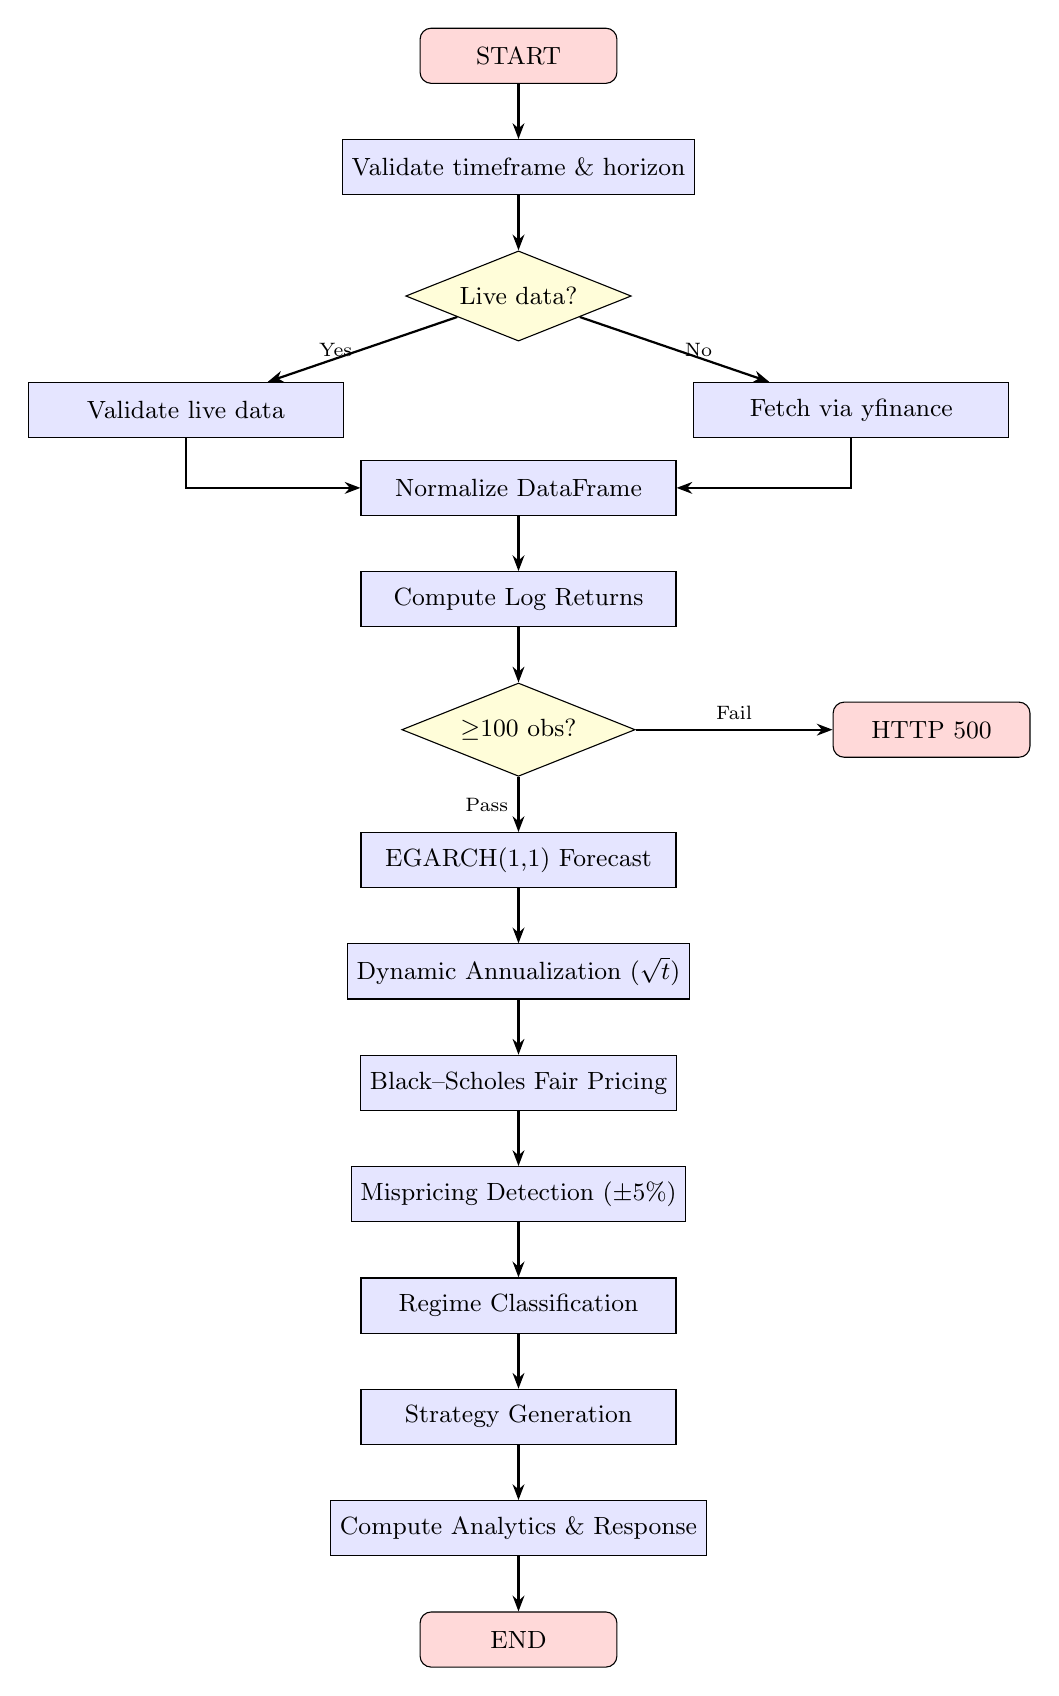
\begin{tikzpicture}[
    node distance=0.7cm,
    startstop/.style={draw, rounded corners, fill=red!15, minimum width=2.5cm, minimum height=0.7cm, align=center, font=\small},
    process/.style={draw, fill=blue!10, minimum width=4cm, minimum height=0.7cm, align=center, font=\small},
    decision/.style={draw, diamond, fill=yellow!15, minimum width=2cm, minimum height=1cm, align=center, font=\small, aspect=2.5},
    arrow/.style={-{Stealth[length=2mm]}, thick}
]

\node[startstop] (start) {START};
\node[process, below=of start] (validate) {Validate timeframe \& horizon};
\node[decision, below=of validate] (live) {Live data?};
\node[process, below left=0.8cm and 1.5cm of live] (vlive) {Validate live data};
\node[process, below right=0.8cm and 1.5cm of live] (vhist) {Fetch via yfinance};
\node[process, below=1.5cm of live] (norm) {Normalize DataFrame};
\node[process, below=of norm] (logreturns) {Compute Log Returns};
\node[decision, below=of logreturns] (checkret) {$\geq$100 obs?};
\node[process, below=of checkret] (egarch) {EGARCH(1,1) Forecast};
\node[process, below=of egarch] (annual) {Dynamic Annualization ($\sqrt{t}$)};
\node[process, below=of annual] (bs) {Black--Scholes Fair Pricing};
\node[process, below=of bs] (misp) {Mispricing Detection ($\pm$5\%)};
\node[process, below=of misp] (regime) {Regime Classification};
\node[process, below=of regime] (strat) {Strategy Generation};
\node[process, below=of strat] (analytics) {Compute Analytics \& Response};
\node[startstop, below=of analytics] (end) {END};

% Error node
\node[startstop, right=2.5cm of checkret] (err) {HTTP 500};

% Arrows
\draw[arrow] (start) -- (validate);
\draw[arrow] (validate) -- (live);
\draw[arrow] (live) -- node[left, font=\scriptsize] {Yes} (vlive);
\draw[arrow] (live) -- node[right, font=\scriptsize] {No} (vhist);
\draw[arrow] (vlive) |- (norm);
\draw[arrow] (vhist) |- (norm);
\draw[arrow] (norm) -- (logreturns);
\draw[arrow] (logreturns) -- (checkret);
\draw[arrow] (checkret) -- node[left, font=\scriptsize] {Pass} (egarch);
\draw[arrow] (checkret) -- node[above, font=\scriptsize] {Fail} (err);
\draw[arrow] (egarch) -- (annual);
\draw[arrow] (annual) -- (bs);
\draw[arrow] (bs) -- (misp);
\draw[arrow] (misp) -- (regime);
\draw[arrow] (regime) -- (strat);
\draw[arrow] (strat) -- (analytics);
\draw[arrow] (analytics) -- (end);

\end{tikzpicture}
\caption{Flowchart of the quantitative analysis pipeline}
\label{fig:flowchart}
\end{figure}

The flowchart describes the logical workflow followed by the system. Starting from input validation, the data undergoes fetching, normalization, log return computation, EGARCH volatility forecasting, annualization, Black--Scholes pricing, mispricing detection, regime classification, and strategy generation. Validation checkpoints are placed throughout the pipeline to ensure data integrity.

\subsection{Class Diagram}

\begin{figure}[H]
\centering
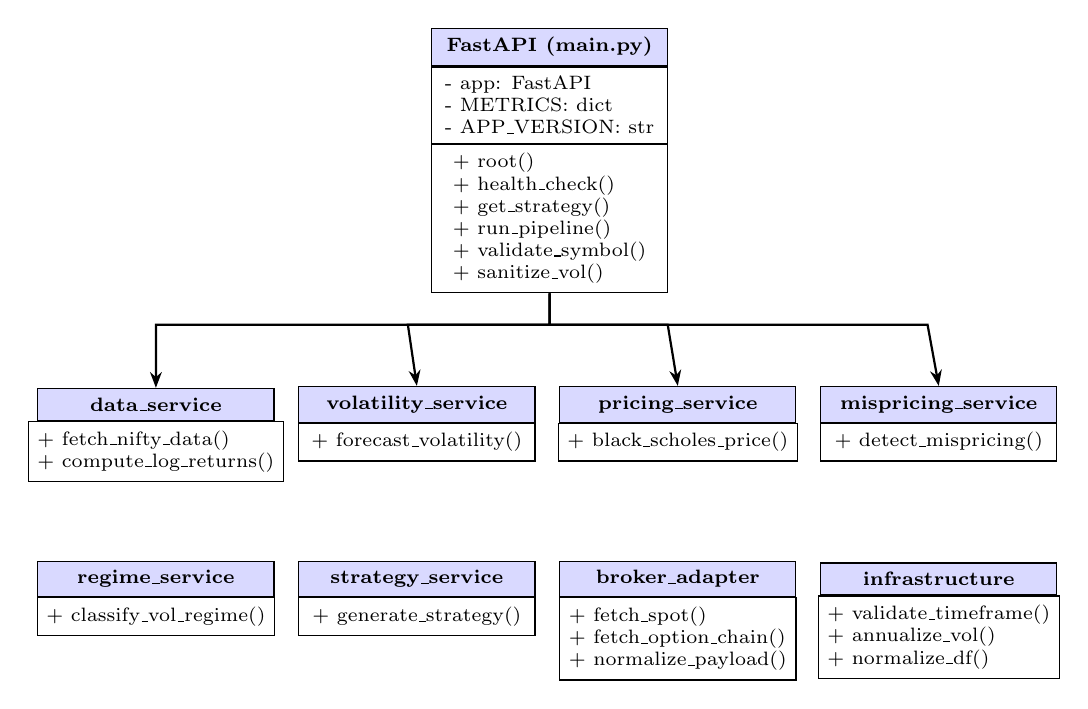
\begin{tikzpicture}[
    node distance=0.6cm and 0.4cm,
    class/.style={draw, minimum width=3cm, align=left, font=\scriptsize},
    classname/.style={draw, fill=blue!15, minimum width=3cm, align=center, font=\scriptsize\bfseries},
    arrow/.style={-{Stealth[length=2mm]}, thick}
]

% Main class
\node[classname] (mainname) at (0, 0) {FastAPI (main.py)};
\node[class, below=0pt of mainname] (mainattr) {- app: FastAPI\\- METRICS: dict\\- APP\_VERSION: str};
\node[class, below=0pt of mainattr] (mainmeth) {+ root()\\+ health\_check()\\+ get\_strategy()\\+ run\_pipeline()\\+ validate\_symbol()\\+ sanitize\_vol()};

% Service classes - row below
\node[classname, below=1.2cm of mainmeth, xshift=-5cm] (dsname) {data\_service};
\node[class, below=0pt of dsname] (dsmeth) {+ fetch\_nifty\_data()\\+ compute\_log\_returns()};

\node[classname, right=0.3cm of dsname] (vsname) {volatility\_service};
\node[class, below=0pt of vsname] (vsmeth) {+ forecast\_volatility()};

\node[classname, right=0.3cm of vsname] (psname) {pricing\_service};
\node[class, below=0pt of psname] (psmeth) {+ black\_scholes\_price()};

\node[classname, right=0.3cm of psname] (msname) {mispricing\_service};
\node[class, below=0pt of msname] (msmeth) {+ detect\_mispricing()};

% Row 3
\node[classname, below=1cm of dsmeth] (rsname) {regime\_service};
\node[class, below=0pt of rsname] (rsmeth) {+ classify\_vol\_regime()};

\node[classname, right=0.3cm of rsname] (ssname) {strategy\_service};
\node[class, below=0pt of ssname] (ssmeth) {+ generate\_strategy()};

\node[classname, right=0.3cm of ssname] (baname) {broker\_adapter};
\node[class, below=0pt of baname] (bameth) {+ fetch\_spot()\\+ fetch\_option\_chain()\\+ normalize\_payload()};

\node[classname, right=0.3cm of baname] (infname) {infrastructure};
\node[class, below=0pt of infname] (infmeth) {+ validate\_timeframe()\\+ annualize\_vol()\\+ normalize\_df()};

% Arrows
\draw[arrow] (mainmeth.south) -- ++(0,-0.4) -- ++(-5,0) -- (dsname.north);
\draw[arrow] (mainmeth.south) -- ++(0,-0.4) -- ++(-1.8,0) -- (vsname.north);
\draw[arrow] (mainmeth.south) -- ++(0,-0.4) -- ++(1.5,0) -- (psname.north);
\draw[arrow] (mainmeth.south) -- ++(0,-0.4) -- ++(4.8,0) -- (msname.north);

\end{tikzpicture}
\caption{Class diagram representing system components}
\label{fig:classdiagram}
\end{figure}

The class diagram represents the structural design of the system. Core modules include data fetching (data\_service), EGARCH volatility forecasting (volatility\_service), Black--Scholes option pricing (pricing\_service), mispricing detection (mispricing\_service), regime classification (regime\_service), strategy recommendation (strategy\_service), and broker data normalization (broker\_adapter). The infrastructure layer provides timeframe configuration, dataframe normalization, and annualization utilities.

% ================================================================
%                4. DESIGN AND METHODOLOGY
% ================================================================
\newpage
\section{Design and Methodology}

\subsection{System Overview}

The objective of the proposed system is to automatically detect options mispricing in the NIFTY~50 index market and provide interpretable strategy recommendations based on quantitative analysis. The system takes market data as input and outputs a comprehensive analytics payload including volatility forecast, fair price, mispricing classification, regime label, strategy recommendation, and supporting diagnostics.

The overall architecture consists of four major modules:

\begin{enumerate}
    \item Market Data Fetching, Preprocessing, and Log Return Computation
    \item EGARCH(1,1) Volatility Forecasting and Dynamic Annualization
    \item Black--Scholes Fair Pricing and Mispricing Detection
    \item Regime Classification and Strategy Recommendation
\end{enumerate}

Figure~\ref{fig:blockdiagram} illustrates the proposed system block diagram.

\begin{figure}[H]
\centering
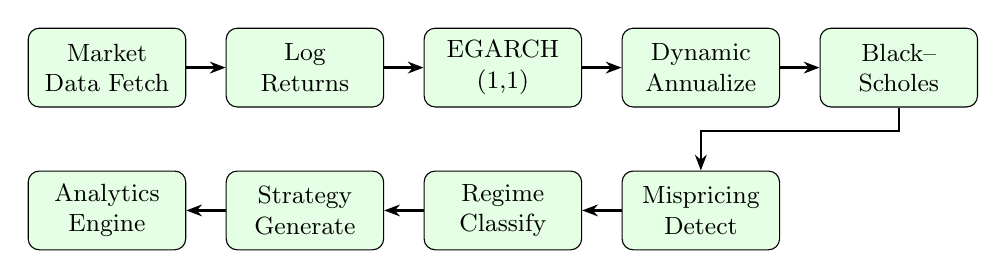
\begin{tikzpicture}[
    node distance=0.3cm and 0.5cm,
    block/.style={draw, rounded corners, fill=green!10, minimum width=2cm, minimum height=1cm, align=center, font=\small},
    arrow/.style={-{Stealth[length=2mm]}, thick}
]

\node[block] (fetch) {Market\\Data Fetch};
\node[block, right=of fetch] (returns) {Log\\Returns};
\node[block, right=of returns] (egarch) {EGARCH\\(1,1)};
\node[block, right=of egarch] (annual) {Dynamic\\Annualize};
\node[block, right=of annual] (bs) {Black--\\Scholes};

\node[block, below=0.8cm of fetch] (analytics) {Analytics\\Engine};
\node[block, right=of analytics] (strat) {Strategy\\Generate};
\node[block, right=of strat] (regime) {Regime\\Classify};
\node[block, right=of regime] (misp) {Mispricing\\Detect};

\draw[arrow] (fetch) -- (returns);
\draw[arrow] (returns) -- (egarch);
\draw[arrow] (egarch) -- (annual);
\draw[arrow] (annual) -- (bs);
\draw[arrow] (bs.south) -- ++(0,-0.3) -| (misp.north);
\draw[arrow] (misp) -- (regime);
\draw[arrow] (regime) -- (strat);
\draw[arrow] (strat) -- (analytics);

\end{tikzpicture}
\caption{Block diagram of the proposed options mispricing detection system}
\label{fig:blockdiagram}
\end{figure}

\subsection{Dataset Used}

The system operates on NIFTY~50 (\texttt{\^{}NSEI}) market data fetched from Yahoo Finance via the yfinance library. The dataset contains OHLCV (Open, High, Low, Close, Volume) data at multiple timeframes. For live deployment, the DhanHQ broker API provides real-time intraday candles and option chain data.

The pipeline requires a minimum of 2,000 candles per timeframe for robust EGARCH estimation, with at least 100 data points after log return computation for stable volatility forecasting.

The recordings correspond to the market trading sessions on NSE, ensuring uniform data conditions across timeframes.

\begin{table}[H]
\centering
\caption{Summary of NIFTY 50 Market Dataset}
\label{tab:dataset}
\begin{tabular}{l l}
\toprule
\textbf{Parameter} & \textbf{Value} \\
\midrule
Underlying Asset & NIFTY 50 Index (\texttt{\^{}NSEI}) \\
Data Provider (Historical) & Yahoo Finance (yfinance) \\
Data Provider (Live) & DhanHQ Broker API \\
Minimum Candles Required & 2,000 per timeframe \\
Minimum EGARCH Observations & 100 log returns \\
Supported Timeframes & 1m, 5m, 15m, 1h, daily, weekly \\
Data Fields & Date, Open, High, Low, Close, Volume \\
Index Timezone & Asia/Kolkata (IST) \\
Risk-Free Rate (assumed) & 6\% (Indian govt.\ bond rate) \\
Option Type (default) & European Call (ATM) \\
\bottomrule
\end{tabular}
\end{table}

The dataset is dynamically fetched based on the requested timeframe with appropriate historical windows (e.g., 7 days for 1-minute, 10 years for daily, max available for weekly).

\subsection{Design and Methodology 1: Market Data Fetching and Log Return Computation}

The input stage handles data acquisition and preprocessing. The \texttt{data\_service} module maps ticker symbols to provider-specific identifiers (e.g., ``NIFTY'' $\rightarrow$ ``\texttt{\^{}NSEI}'' for yfinance), selects appropriate fetch windows based on the requested timeframe, and downloads OHLCV data with automatic adjustment for corporate actions.

The \texttt{timeframe\_adapter} module then normalizes the raw dataframe by:

\begin{itemize}
    \item Validating required columns (Date, Open, High, Low, Close, Volume)
    \item Converting dates to datetime format
    \item Sorting chronologically and removing duplicate timestamps
    \item Forward-filling missing values
    \item Ensuring numeric dtypes for OHLCV columns
\end{itemize}

Log returns are computed as:
\begin{equation}
    r_t = \ln\left(\frac{C_t}{C_{t-1}}\right)
\end{equation}
where $C_t$ is the closing price at time $t$. Log returns are preferred over simple returns due to their additive property across time periods and approximate normality for small returns.

\subsection{Design and Methodology 2: EGARCH Volatility Forecasting and Annualization}

The volatility forecasting module implements the EGARCH(1,1) model proposed by Nelson (1991) [10]. The log returns are scaled to percentage form (multiplied by 100) before fitting the model.

The EGARCH(1,1) conditional variance equation (in log form) is:
\begin{equation}
    \ln(\sigma_t^2) = \omega + \alpha \left(\frac{|\varepsilon_{t-1}|}{\sigma_{t-1}} - \sqrt{\frac{2}{\pi}}\right) + \gamma \frac{\varepsilon_{t-1}}{\sigma_{t-1}} + \beta \ln(\sigma_{t-1}^2)
\end{equation}
where $\omega$ is the constant, $\alpha$ captures the magnitude effect, $\gamma$ captures the asymmetric (leverage) effect, and $\beta$ captures volatility persistence.

The model is fitted using maximum likelihood estimation via the \texttt{arch} library with normal distribution assumed for innovations. One-step-ahead conditional variance forecast is extracted, and the forecasted volatility (standard deviation) is converted from percentage scale back to decimal.

\textbf{Dynamic Annualization.} The \texttt{annualization\_engine} applies the square root of time scaling rule:
\begin{equation}
    \sigma_\text{annual} = \sigma_\text{period} \times \sqrt{N}
\end{equation}
where $N$ is the number of periods per year (e.g., $N = 252$ for daily, $N = 252 \times 78 = 19{,}656$ for 5-minute).

\textbf{Volatility Sanitization.} The sanitized volatility is clamped to $[0.01, 2.0]$ (1\%--200\%) with NaN/infinity fallback to 0.15 (15\%).

\textbf{Horizon Adjustment.} A trading horizon multiplier scales the volatility for interpretation:
\begin{itemize}
    \item Day Trader: $\times 1.15$ (short-term sensitive)
    \item Positional: $\times 1.0$ (balanced)
    \item Long-Term: $\times 0.85$ (smoothed)
\end{itemize}

\subsection{Design and Methodology 3: Black--Scholes Fair Pricing and Mispricing Detection}

The Black--Scholes model computes the theoretical fair value for a European call option:
\begin{equation}
    C = S \cdot N(d_1) - K \cdot e^{-rT} \cdot N(d_2)
\end{equation}
where:
\begin{equation}
    d_1 = \frac{\ln(S/K) + (r + \sigma^2/2) \cdot T}{\sigma\sqrt{T}}, \qquad d_2 = d_1 - \sigma\sqrt{T}
\end{equation}

\begin{itemize}
    \item $S$ = spot price (from latest close or live broker data)
    \item $K$ = strike price (set to ATM, i.e., $K = S$)
    \item $T$ = time to expiry in years (parsed from option chain or default 0.1 years)
    \item $r$ = risk-free rate (0.06, Indian government bond rate)
    \item $\sigma$ = horizon-adjusted, expiry-scaled volatility from EGARCH
    \item $N(\cdot)$ = cumulative standard normal distribution (\texttt{scipy.stats.norm.cdf})
\end{itemize}

The mispricing detection module compares the observed market price against the Black--Scholes fair value:
\begin{equation}
    \text{deviation} = \frac{P_\text{market} - P_\text{fair}}{P_\text{fair}}
\end{equation}

Classification is based on a $\pm$5\% threshold:
\begin{itemize}
    \item \textbf{Overpriced:} deviation $> +5\%$
    \item \textbf{Fair:} $-5\% \leq$ deviation $\leq +5\%$
    \item \textbf{Underpriced:} deviation $< -5\%$
\end{itemize}

\subsection{Design and Methodology 4: Regime Classification and Strategy Generation}

\textbf{Volatility Regime Classification} uses threshold-based rules on the annualized volatility forecast:

\begin{table}[H]
\centering
\begin{tabular}{l l}
\toprule
\textbf{Regime} & \textbf{Volatility Range} \\
\midrule
LOW\_VOL & $\sigma < 15\%$ \\
NORMAL\_VOL & $15\% \leq \sigma < 25\%$ \\
HIGH\_VOL & $25\% \leq \sigma < 40\%$ \\
EXTREME\_VOL & $\sigma \geq 40\%$ \\
\bottomrule
\end{tabular}
\end{table}

\textbf{Strategy Generation} uses a rule-based mapping that combines mispricing classification with the volatility regime. The 12-cell strategy matrix (3 mispricing states $\times$ 4 regime states) produces specific recommendations:

\begin{table}[H]
\centering
\small
\begin{tabularx}{\textwidth}{l X X X X}
\toprule
\textbf{Mispricing $\backslash$ Regime} & \textbf{LOW\_VOL} & \textbf{NORMAL\_VOL} & \textbf{HIGH\_VOL} & \textbf{EXTREME\_VOL} \\
\midrule
\textbf{Underpriced} & Long volatility (high) & Buy options (med) & Buy with caution (med) & Wait for stability (low) \\
\textbf{Fair} & No strong edge (low) & No strong edge (low) & Fairly priced (low) & Wait for opportunity (low) \\
\textbf{Overpriced} & Sell premium cautiously (med) & Sell premium (med) & Credit spread (high) & High risk short vol (med) \\
\bottomrule
\end{tabularx}
\end{table}

\begin{table}[H]
\centering
\caption{Evaluation Metrics}
\label{tab:eval_metrics}
\begin{tabularx}{\textwidth}{l X}
\toprule
\textbf{Metric} & \textbf{Description} \\
\midrule
Pipeline Health & OK if volatility $> 0$ and fair\_price $> 0$; CHECK\_DATA otherwise \\
Confidence Score & $\min(1.0,\; |\text{deviation}| \times 5)$; thresholds: $\geq 0.7$ Strong, $\geq 0.4$ Moderate, else Weak \\
Signal Strength & $|\text{deviation}| \times \sigma_\text{forecast}$ \\
Regime Confidence & Distance from nearest boundary / (regime width / 2) \\
Quant Stability & (validation flags avg) $\times$ signal strength normalized \\
Analytics Health & 1.0 baseline, penalized for pipeline issues and low confidence \\
\bottomrule
\end{tabularx}
\end{table}

% ================================================================
%                       REFERENCES
% ================================================================
\newpage
\begin{thebibliography}{99}

\bibitem{black1973}
F.~Black and M.~Scholes, ``The Pricing of Options and Corporate Liabilities,'' \textit{Journal of Political Economy}, vol.~81, no.~3, pp.~637--654, 1973.

\bibitem{andersen1998}
T.~G.~Andersen and T.~Bollerslev, ``Answering the Skeptics: Yes, Standard Volatility Models Do Provide Accurate Forecasts,'' \textit{International Economic Review}, vol.~39, no.~4, pp.~885--905, 1998.

\bibitem{bollerslev1986}
T.~Bollerslev, ``Generalized Autoregressive Conditional Heteroskedasticity,'' \textit{Journal of Econometrics}, vol.~31, no.~3, pp.~307--327, 1986.

\bibitem{engle1982}
R.~F.~Engle, ``Autoregressive Conditional Heteroscedasticity with Estimates of the Variance of United Kingdom Inflation,'' \textit{Econometrica}, vol.~50, no.~4, pp.~987--1007, 1982.

\bibitem{christoffersen2004}
B.~J.~Christoffersen and K.~Jacobs, ``The Importance of the Loss Function in Option Valuation,'' \textit{Journal of Financial Economics}, vol.~72, no.~2, pp.~291--318, 2004.

\bibitem{duan1995}
J.~C.~Duan, ``The GARCH Option Pricing Model,'' \textit{Mathematical Finance}, vol.~5, no.~1, pp.~13--32, 1995.

\bibitem{bucci2020}
A.~Bucci, ``Realized Volatility Forecasting with Neural Networks,'' \textit{Journal of Financial Econometrics}, vol.~18, no.~3, pp.~502--531, 2020.

\bibitem{karmakar2005}
M.~Karmakar, ``Modeling Conditional Volatility of the Indian Stock Markets,'' \textit{Vikalpa}, vol.~30, no.~3, pp.~21--37, 2005.

\bibitem{hansen2005}
P.~R.~Hansen and A.~Lunde, ``A Forecast Comparison of Volatility Models: Does Anything Beat a GARCH(1,1)?,'' \textit{Journal of Applied Econometrics}, vol.~20, no.~7, pp.~873--889, 2005.

\bibitem{nelson1991}
D.~B.~Nelson, ``Conditional Heteroskedasticity in Asset Returns: A New Approach,'' \textit{Econometrica}, vol.~59, no.~2, pp.~347--370, 1991.

\bibitem{baillie1996}
R.~T.~Baillie, T.~Bollerslev, and H.~O.~Mikkelsen, ``Fractionally Integrated Generalized Autoregressive Conditional Heteroskedasticity,'' \textit{Journal of Econometrics}, vol.~74, no.~1, pp.~3--30, 1996.

\bibitem{hull2018}
J.~C.~Hull, \textit{Options, Futures, and Other Derivatives}, 10th~ed. Pearson, 2018.

\bibitem{liu2019}
S.~Liu, A.~Borovykh, L.~A.~Grzelak, and C.~W.~Oosterlee, ``A Neural Network-Based Framework for Financial Model Calibration,'' \textit{Journal of Mathematics in Industry}, vol.~9, art.~9, 2019.

\bibitem{wilmott2006}
P.~Wilmott, \textit{Paul Wilmott on Quantitative Finance}, 2nd~ed. Wiley, 2006.

\bibitem{tripathy2015}
T.~Tripathy and L.~A.~Gil-Alana, ``Modelling Time-Varying Volatility in the Indian Stock Returns: Some Empirical Evidence,'' \textit{Review of Development Finance}, vol.~5, no.~2, pp.~91--97, 2015.

\bibitem{lopezdeprado2018}
M.~L\'{o}pez~de~Prado, \textit{Advances in Financial Machine Learning}. Wiley, 2018.

\bibitem{chan2013}
E.~Chan, \textit{Algorithmic Trading: Winning Strategies and Their Rationale}. Wiley, 2013.

\end{thebibliography}

\end{document}
